\section{Code Analyse}
\subsection{Datenfluss Analyse}
\begin{itemize}
    \item Mächtige und generische Code-Analyse-Technik
    \item Für viele Optimierungen nützlich
\end{itemize}
\subsubsection{Analysebeispiele}
\begin{itemize}
    \item Wo werden uninitialisierte Variablen gelesen?
    \item Ist der Wert einer Variable konstant?
    \item \textbf{Alle Pfade analysieren}
\end{itemize}
\subsubsection{Ansatz}
\textbf{Control Flow Graph erstellen}
\begin{itemize}
    \item Zeigt alle Programm-Pfade
\end{itemize}
\textbf{Datenfluss-Analyse durchführen}
\begin{itemize}
    \item Propagiere Information durch den Graph, bis es stabil ist
\end{itemize}

\subsection{Control Flow Graph}
\begin{itemize}
    \item Repräsentiert alle möglichen Programmpfade (Typischerweise innerhalb einer Methode)
    \item Knoten = Basic Block
    \begin{itemize}
        \item Unterbrochener Code-Abschnitt
        \item Einstieg nur am Anfang: Kein Label in der Mitte
        \item Ausstieg nur am Schluss: Kein Branch in der Mitte
    \end{itemize}
    \item Kante
    \begin{itemize}
        \item Bedingter oder unbedingter Branch
    \end{itemize}
\end{itemize}

\subsubsection{Basic Blocks}
\begin{itemize}
    \item Grenzen durch Branch Entries/Exits gegeben
\end{itemize}
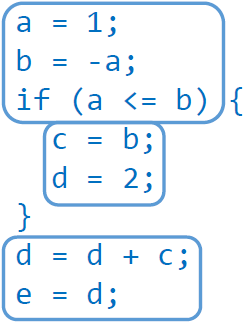
\includegraphics[width=0.2\linewidth]{basic_blocks.png}

\subsubsection{Verknüpfung}
\begin{itemize}
    \item Basic Blocks nach möglichen Branches verknüpfen
\end{itemize}
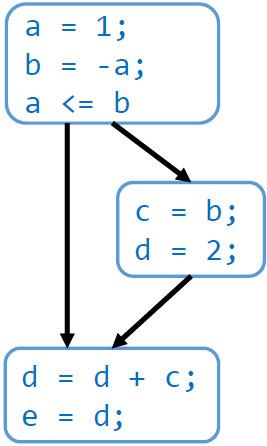
\includegraphics[width=0.2\linewidth]{cfg.png}

\subsubsection{If-Statement}
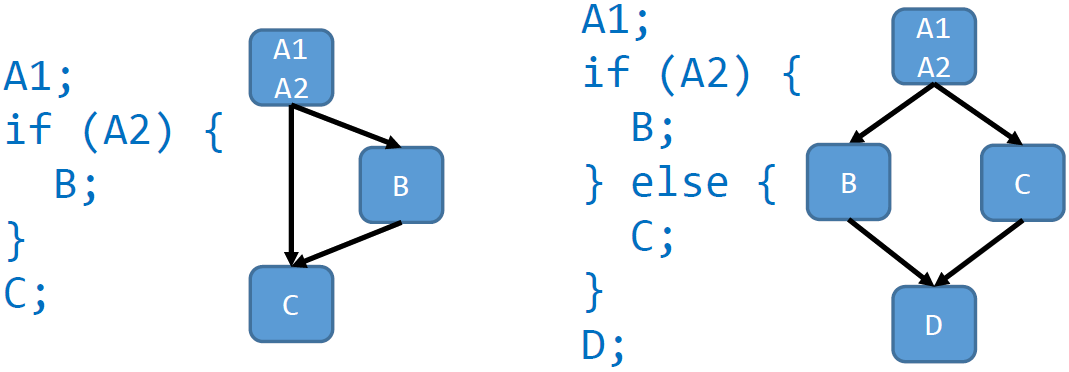
\includegraphics[width=0.5\linewidth]{cfg_if.png}

\subsubsection{While-Statement}
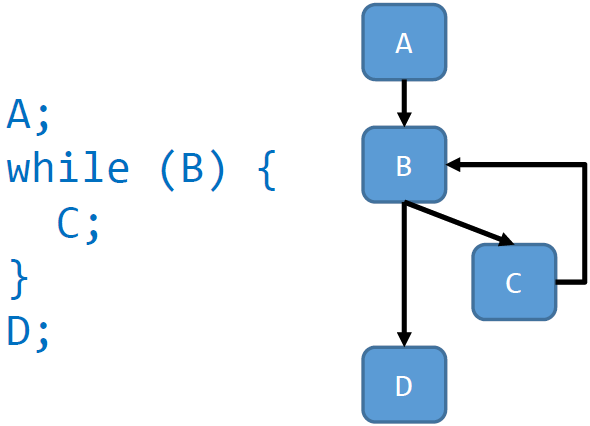
\includegraphics[width=0.4\linewidth]{cfg_while.png}

\subsection{Datenflussanalyse}
\begin{itemize}
    \item Fixpunkt-Iteration über CFG
    \begin{itemize}
        \item Propagiere Analyse-Information über Blöcke
        \item Bis es für jeden Block stabil ist
    \end{itemize}
    \item Generische Methode
    \begin{itemize}
        \item Verschiedene Anwendungsfälle
        \item Wird fallspezifisch konfiguriert
    \end{itemize}
\end{itemize}

\subsubsection{State}
\begin{itemize}
    \item Input State und Output State pro Basic Block
    \item Analyse-Information vor und nach einem Block
\end{itemize}

\subsubsection{Transfer}
\begin{itemize}
    \item Abbildung pro Block: Input State $\rightarrow$ Output State
    \item Definiert, was der Block auf Zustand bewirkt
\end{itemize}

\subsubsection{Beispiel}
\begin{itemize}
    \item State = Menge der uninitialisierten Variablen
    \item Transfer = Füge Deklarationen dazu, entferne zugewiesene Variablen
\end{itemize}
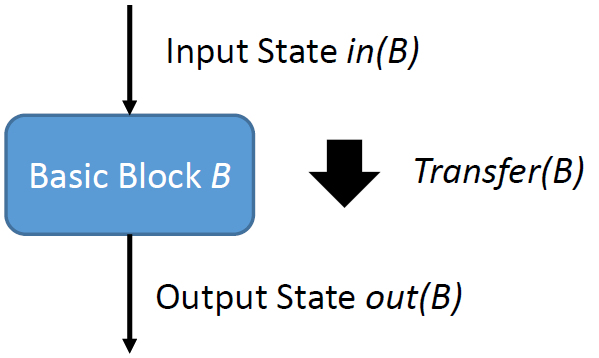
\includegraphics[width=0.4\linewidth]{bsp1.png}
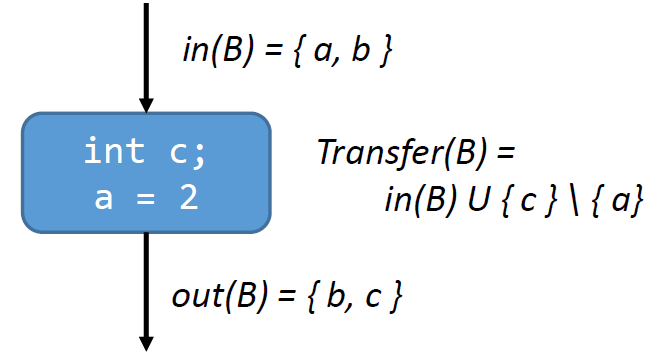
\includegraphics[width=0.4\linewidth]{bsp2.png}

\subsubsection{Join}
\begin{itemize}
    \item Kombiniere Output States der Vorgänger zu Input State eines Nachfolgers
    \item Vereinigungsmenge der Vorgänger
\end{itemize}
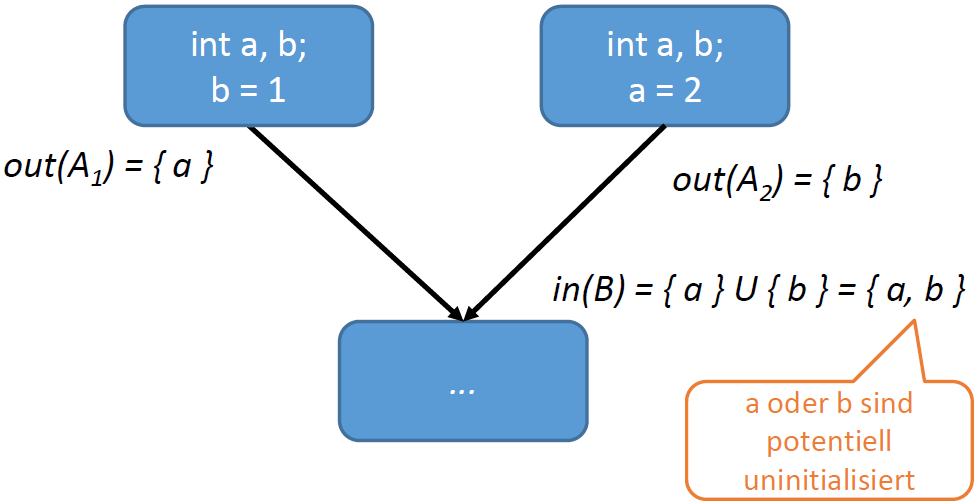
\includegraphics[width=0.4\linewidth]{join.png}

\subsubsection{Code}
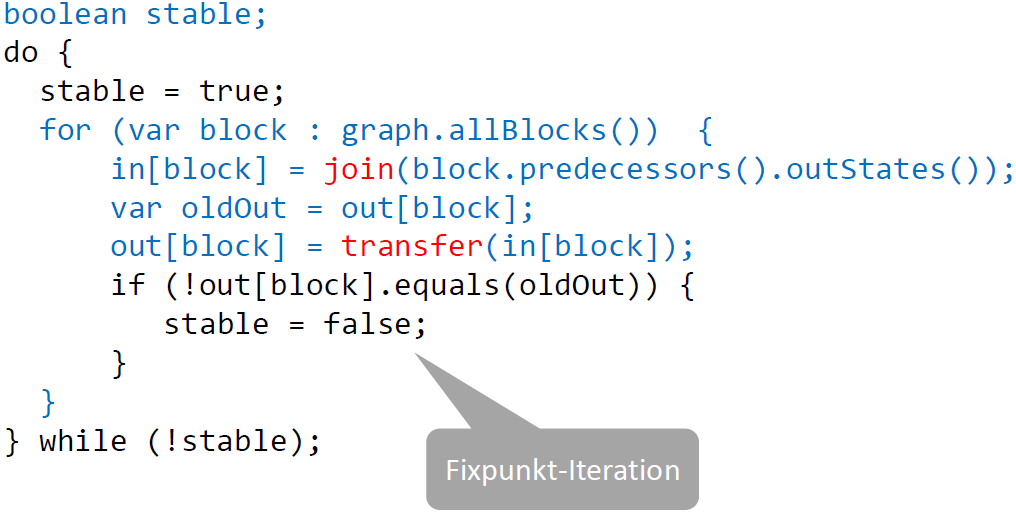
\includegraphics[width=0.5\linewidth]{datenflussanalyse.png}

\subsubsection{Resultat ableiten}
\begin{itemize}
    \item Stabiler Input oder Output State benutzen
    \item z.B. Compiler-Fehler für uninitialisiertes Lesen
\end{itemize}

\subsection{Diskussion}
\textbf{Konservative Analyse}
\begin{itemize}
    \item Betrachtet alle möglichen syntaktischen Pfade
\end{itemize}
\textbf{Kontextfreie Analyse}
\begin{itemize}
    \item Alle Pfade werden gewählt, egal ob Bedingung erfüllt ist
\end{itemize}
\textbf{Fehlermeldung ist auch konservativ}
\begin{itemize}
    \item Falls mindestens ein Pfad mit Fehler existiert = Error
\end{itemize}
\textbf{Fixpunkt-Iteration muss terminieren}
\begin{itemize}
    \item z.B. Falls Menge monoton mit Joins wächst
\end{itemize}
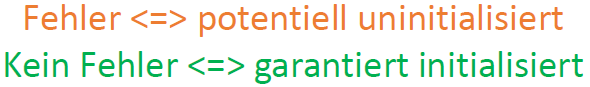
\includegraphics[width=0.3\linewidth]{diskussion.png}

\subsection{Andere Anwendung}
\textbf{Constant Propagation}
\begin{itemize}
    \item Konstante Werte bei Transfer merken
    \item Join = Intersection
\end{itemize}
\textbf{Rückwärts-Propagierung}
\begin{itemize}
    \item Transfer: Out State $\rightarrow$ In State
    \item z.B. Für Dead Code Analysis
\end{itemize}